\documentclass{article}
\usepackage[utf8]{inputenc}
\usepackage[margin=0.5in]{geometry}

\title{HW2\_ClassNote}
\author{Group2: Yaxin Li, Blake Hillier, Joe Puhalla}
\date{January 2020}

\usepackage{natbib}
\usepackage{graphicx}

\usepackage{amsmath, amssymb, amsthm}


\begin{document}

\maketitle

Claim: Average of 2 O.N. matrix may not be an O.N. matrix.
\begin{align*}
    AA^{T} &= I \\
    BB^{T} &= I \\
    M &= \frac{(A+B)}{2} \\
    MM^{T} &= (\frac{A+B}{2})(\frac{A^{T}+B^{T}}{2}) \\
        &= \frac{1}{4}\ [\ AA^{T}+AB^{T}+BA^{T}+BB^{T} \ ] \\
        &=I
\end{align*}

Use time. Collect data from Jan 2020 to Now.\\

Use only stocks. Let's say pick 3 stocks out of 3000 stocks from different sectors such as Fiance, Tech, Real Estate, Health and so on. Each group takes 100 stocks.

\begin{align*}
    \text{Make}\ \sigma &= \begin{bmatrix}
           \sigma_{1} \\
           \sigma_{2} \\
           %\vdots \\ 
           \sigma_{3}
         \end{bmatrix}
\end{align*}

$\text{Get} S_{k}, S_{l}, S_{m} \text{from the following matrix}$

\begin{align*}
  M=
  \left[ {\begin{array}{ccccc}
   \vdots & \vdots & \vdots \\
   P_{sk}^2 & P_{sl}^2 & P_{sm}^2 \\
   \vdots & \vdots & \vdots \\
  \end{array} } \right] = Z_{N\times3}
\end{align*}

Draw the picture as following\\
\graphicspath{ {./images/} }

\begin{wrapfigure}{r}
    \resizebox{8cm}{!}{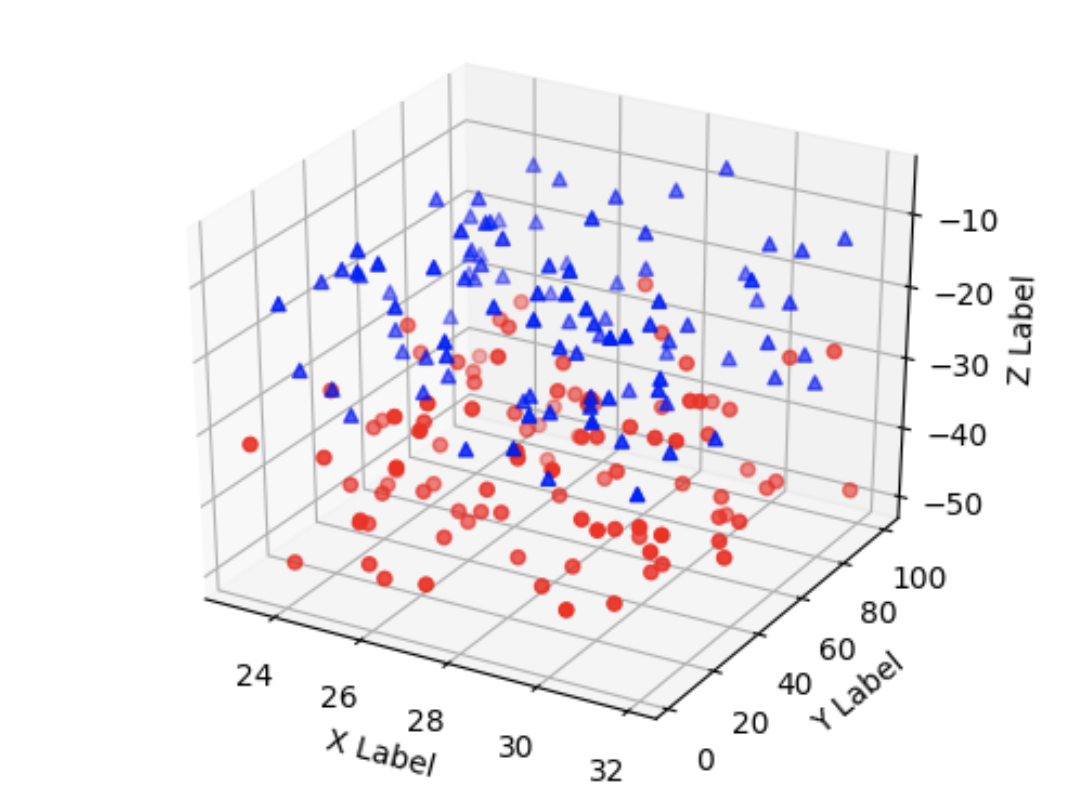
\includegraphics{111.png}}
\end{wrapfigure}

\end{document}
